\documentclass[12pt]{article}

\usepackage[utf8]{inputenc}
\usepackage[T1]{fontenc}
\usepackage[brazilian]{babel}
\usepackage{cancel}

\usepackage{geometry}
\geometry{margin=2.5cm}
\usepackage{setspace}
\onehalfspacing

\usepackage{amsmath, amssymb, amsthm}
\usepackage{mathtools}

\numberwithin{equation}{section}

\theoremstyle{plain}
\newtheorem{theorem}{Teorema}[section]
\newtheorem{proposition}[theorem]{Proposição}
\newtheorem{lemma}[theorem]{Lema}
\newtheorem{corollary}[theorem]{Corolário}

\theoremstyle{definition}
\newtheorem{definition}[theorem]{Definição}
\newtheorem{example}[theorem]{Exemplo}
\newtheorem{exercise}{Exercício}

\theoremstyle{remark}
\newtheorem*{remark}{Observação}

\usepackage{hyperref}
\hypersetup{hidelinks}
\usepackage{csquotes}

\usepackage[
    backend=biber,
    style=abnt
]{biblatex}

\addbibresource{../Microeconomics.bib}

\newcommand{\R}{\mathbb{R}}
\newcommand{\pref}{\succeq}
\newcommand{\strictpref}{\succ}
\newcommand{\indiff}{\sim}

% ------------------------------------------------
% Title (fill manually)
% ------------------------------------------------
\title{Lista 3 --- Teoria Microeconômica (PPGE-UFF)}
\author{Professor: Fábio Waltenberg\thanks{\href{mailto:fdwaltenberg@id.uff.br}{fdwaltenberg@id.uff.br}} \\Monitor: Nicholas Funari Voltani\thanks{\href{mailto:nicholasvoltani@gmail.com}{nicholasvoltani@gmail.com}}}
\date{}

\begin{document}
\maketitle

\section{Conceitos introdutórios}
\subsection{Identidades matemáticas em Teoria do Consumidor}
Resultados importantes para a teoria do consumidor, assim como para a teoria da firma, são o lema de Shephard e a identidade de Roy.\footnote{Suas demonstrações são mais convolutas. Para o leitor interessado: suas demonstrações giram em torno do \textit{envelope theorem}, e recomendo singelamente minha demonstração destes resultados em \href{https://nicholasvoltani.github.io/Envelope-Theorem}{[[Envelope Theorem]]}.}

O lema de Shephard associa a demanda hicksiana \(\vec{h}(\vec{p}, \bar{u})\) com a função dispêndio \(e(\vec{p}, \bar{u})\): a trajetória da demanda hicksiana é descrita pela variação do dispêndio com relação aos \textit{preços}. Formalmente:
\[
\nabla_{p} {e(\vec{p}, \bar{u})} = \vec{h}(p, \bar{u}) 
\]

A identidade de Roy é um corolário do lema de Shephard, resultado obtido pela derivação da função de utilidade indireta:
\[
\nabla_{p} v\left(\vec{p}, e(\vec{p}, \bar{u})\right) = \nabla_{p} \underbrace{\bar{u}}_{\text{Constante!}} = 0
\]

Portanto, a identidade de Roy tem a forma
\[
\vec{h}(p, \bar{u}) = -\frac{1}{\left( \frac{ \partial v }{ \partial w } \right) } \nabla_{p}v
\]
Ou, escrevendo para cada bem $i$,
\[
h_i(p, \bar{u}) = -\frac{\left( \frac{ \partial v }{ \partial p_i } \right) }{\left( \frac{ \partial v }{ \partial w } \right) } 
\]


\subsection{Loterias}
No contexto de Microeconomia, uma loteria não é mais do que uma lista de valores $L = (p_1, \dots, p_n)$ tal que 
\[
\sum\limits_{i=1}^n p_i = 1 
\]
Ou seja, $L$ é, por assim dizer, um vetor de probabilidades, em que cada $i = 1, \dots, n$ representa algo de interesse, seja p. ex. um bem, ou mesmo uma outra loteria.

\begin{figure}[h]
  \centering
  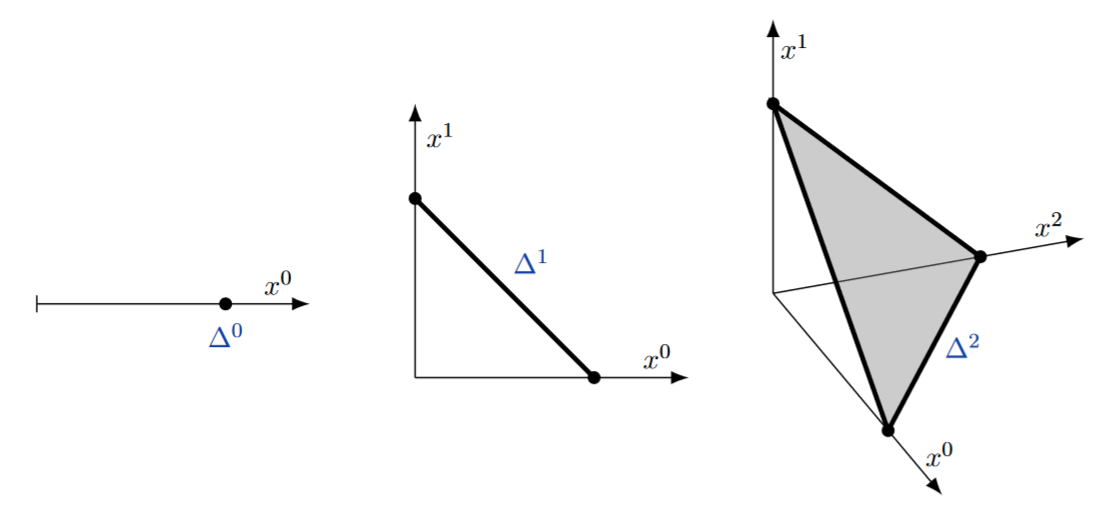
\includegraphics[width=0.8\textwidth]{images/simplexos.png}
  \caption{Representação gráfica de simplexos de $0$ (caso trivial, não-pertinente), $1$ e $2$ dimensões --- no que nos diz respeito, loterias de $1$, $2$ e $3$ argumentos. Note que, embora um $n$-simplexo seja $n$-dimensional (resp. acima: um ponto, uma reta e um plano), sua visualização em $\mathbb{R}^{n+1}$ ilustra melhor como a normalização $\sum\limits_i p_i = 1$ aparece. Fonte: \href{https://ncatlab.org/nlab/show/simplex}{https://ncatlab.org/nlab/show/simplex}.}
\end{figure}


É possível visualizá-lo no que se chama de \textit{simplexos}. Por clareza, pensemos que cada componente de uma loteria $L$ se trata de algum bem, e $p_i$ é alguma probabilidade a ele associada. Então, um simplexo de duas dimensões --- associado a uma loteria $L = (p_1, p_2)$ --- seria meramente um segmento de reta $[0,1] \subset \mathbb{R}$ em que os extremos representam cada bem; usualmente pensamos em $p \in [0, 1]$, porém isso é o mesmo que dizer que $p$ é a probabilidade \textit{do bem da extremidade direita} --- denotemos ele por $p_2$ ---, e $1-p$ a probabilidade \textit{do bem da extremidade esquerda} --- denotemos ele por $p_1$.\footnote{O motivo que é possível descrever essa loteria por um número somente é justamente pela restrição de normalização $\sum\limits_i p_i$. O número de variáveis do problema é $2$ (a quantidade de bens), e possui $1$ restrição (a restrição de normalização); portanto, o problema possui somente $2-1 = 1$ grau de liberdade, i.e. requer somente $1$ variável para sua descrição completa --- no caso acima, $p$. Para loterias de $n$ argumentos, haverá $n-1$ graus de liberdade pelo mesmo motivo.} Dessa forma, temos que o segmento de reta $[0, 1]$ é o simplexo que representa uma loteria $(p_1, p_2)$. Num caso de uma loteria de $3$ bens/argumentos, o simplexo é um triângulo em $\subset \mathbb{R}^2$

\begin{figure}[h]
  \centering
  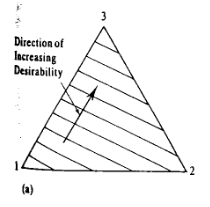
\includegraphics[width=0.4\textwidth]{images/Simplex.png}
  \caption{Representação gráfica de uma loteria com $3$ possibilidades \parencite[p. 175, figura \textbf{6.B.5} a).]{Mas-Colell1995}. Note que as opções, quando individualmente consideradas, têm preferência $1 \prec  2 \prec  3$.}
\end{figure}

\begin{example}[Seguros]
  \label{exemploseguros}
  \parencite[exemplo 6.C.1]{Mas-Colell1995} Considere um tomador de decisão estritamente avesso ao risco que tenha uma riqueza inicial de \(w\), mas que corra o risco de perder \(D\) dólares. A probabilidade de perda é \(\pi\).\footnote{Não, não é \(3.1415 \dots\) P.S.: este $\pi$ não se trata do \textit{probability premium} --- culpe Mas-Collell et al. pelo abuso de notação!!} É possível, entretanto, que o tomador de decisão adquira um seguro. Uma unidade de seguro custa \(q\) dólares e paga \(1\) dólar se a perda ocorrer. Assim, se \(\alpha\) unidades de seguro forem compradas, o patrimônio do indivíduo será \(w-\alpha q\), se não houver sinistro\footnote{Um ``sinistro'' ocorre quando um seguro é acionado devido a uma perda a ser indenizada. O pagamento de um sinistro se chama ``indenização''.} e \(w-\alpha q-D+\alpha\) se o sinistro ocorrer. Observe, para fins de discussão posterior, que a riqueza esperada do tomador de decisão é então \(w - \pi D + \alpha (\pi - q)\). O problema do tomador de decisão é escolher o nível ótimo de \(\alpha\). Seu problema de maximização de utilidade é
    \[
      \max\limits_{\alpha \geq 0}  \,(1-\pi) \, u(w-\alpha q) + \pi u(w-\alpha q - D + \alpha )
  \]
  Se \(\alpha^*\) for ótimo, ele deve satisfazer a condição de primeira ordem:
  \[
    -q(1-\pi) \, u^{\prime} (w-\alpha^* q)+ \pi(1-q) u^{\prime} (w-D+\alpha^* (1-q)) \leq 0
  \]
  com igualdade se \(\alpha^* > 0\).
  
  Suponha agora que o preço \(q\) de uma unidade de seguro seja atuarialmente justo no sentido de ser igual ao custo esperado do seguro. Ou seja, \(q=\pi\). Então a condição de primeira ordem requer que
  \[
  u^{\prime} (w-D+\alpha^* (1-\pi))-u^{\prime} (w-\alpha^* \pi) \leq 0
  \]
  com igualdade se \(\alpha^* > 0\).
  
  Como \(u^\prime (w-D) > u^\prime (w)\), devemos ter \(\alpha^*>0\) e, portanto,
  \[
  u^\prime (w-D+\alpha^* (1-\pi))=u^\prime (w-\alpha^* \pi)
  \]
  
  Como \(u^{\prime}  (\cdot)\) é estritamente decrescente, isso implica
  \[
    w-D+\alpha^* (1-\pi)=w-\alpha^* \pi
    \]
    ou, equivalentemente,
    \[
      \alpha^* = D
      \]
      
      Assim, se o seguro for atuarialmente justo, o tomador de decisão faz seguro completo. A riqueza final do indivíduo é então \(w-\pi D\), independentemente da ocorrência da perda.
      
      Essa prova do resultado do seguro total usa condições de primeira ordem, o que é instrutivo, mas não é realmente necessário. Observe que se \(q=\pi\), então a riqueza esperada do tomador de decisão é \(w-\pi D\) para qualquer \(\alpha\). Como definir \(\alpha=D\) permite que ele alcance \(w-\pi D\) com certeza, a definição de aversão ao risco implica diretamente que este é o nível ótimo de \(\alpha\).
\end{example}
  
\subsection{Um básico de probabilidades condicionais}
Dada uma distribuição de probabilidades $P$, temos que a probabilidade de certo evento $X$ \textit{condicional a certo evento} $I$ é definida como
\[
P(X \mid I) = \frac{P(X \cap I)}{P(I)}
\]

\begin{example}
  Seja P(X) uma distribuição de probabilidade uniforme sobre os valores possíveis de um dado (seja seu espaço amostral $S \coloneqq \{1, 2, 3, 4, 5, 6\}$). Então\footnote{A rigor, como probabilidades são \textit{funções de medida} de subconjuntos do espaço amostral $S$ (a rigor$^2$, de conjuntos em uma $\sigma$-álgebra de $S$), então $P(X=x)$ quer dizer $P(\{x\})$, ou seja, a função probabilidade avaliando a ``medida'' do conjunto $\{x\}$.}
  \[
  \forall x \in \{1, 2, 3, 4, 5, 6\}: P(X = x) = \frac{1}{6} 
  \]
  
  Por exemplo, seja $I$ definida como ``o número tirado no dado é \textit{par}'' --- em termos de conjunto, no caso, $I \coloneqq \{2, 4, 6\}$. Então tem-se que $P(I) = P(2) + P(4) + P(6) = \frac{1}{2}$ (por quê?), e as probabilidades de cada elemento em $S$ condicionais a $I$ são

  \[
  \forall x \in \{1, 2, 3, 4, 5, 6\}: P(X = x \mid I) = \frac{P(\{x\} \cap I)}{P(I)} = \begin{cases}
    0, x \in \{1, 3, 5 \} \\
    \frac{1/6}{1/2} = \frac{1}{3}, x \in \{2, 4, 6\}
  \end{cases}
  \]

  Na prática, o que ocorre é que a probabilidade condicional está agindo sobre um ``espaço amostral menor'': invés de agir sobre o espaço amostral inteiro $S$, ele age sobre $I$, o conjunto pressuposto. De fato, sempre fala-se de probabilidades condicionais; a questão é que $P(S) = 1$ por pressuposto. Mas o que ocorre, mediante uma probabilidade condicional, é que há a mudança
  \[
  P(X) = \frac{P(X)}{P(S)} \mapsto \frac{P(X \cap I)}{P(S \cap I)} = \frac{P(X \cap I)}{P(I)}
  \]
\end{example}

\subsection{Aversão ao risco}
\begin{definition}[\textit{Probability Premium}]
  Dada uma função de utilidade de Bernoulli $u(x)$ de algum tomador de decisão com riqueza inicial $x_0$, ele é indiferente a uma aposta $(x_0 \pm \epsilon)$ com algum $\epsilon > 0$ se, e somente se, ela for associada à loteria $(\frac{1}{2} + \pi(x_0, \epsilon, u), \frac{1}{2} - \pi(x_0, \epsilon, u))$. Equivalentemente, somente quando vale
  \[
  u(x) = \left( \frac{1}{2} + \pi(x, \epsilon, u) \right) u(x + \epsilon) + \left( \frac{1}{2} - \pi(x, \epsilon, u) \right) u(x - \epsilon)
  \]

  $\pi(x_0, \epsilon, u)$ é dito ser seu \textit{probability premium}.\footnote{Não encontrei nome em português. ``Prêmio de risco'' é outra coisa, pois é uma quantidade \textit{monetária}, enquanto $\pi(x_0, \epsilon, u)$ é uma \textit{probabilidade}.} 

\end{definition}

\begin{definition}[Equivalente certo]
  Dada uma função de utilidade de Bernoulli $u(x)$ de algum tomador de decisão, o \textit{equivalente certo} $c(L, u)$ a alguma loteria $L = (p_1, \dots , p_n)$, que diz respeito às possibilidades $x_1, \dots , x_n$, é a quantidade monetária que lhe dá a utilidade esperada (i.e. von Neumann-Morgenstern) relacionada a esta loteria.

  Ou seja, 
  \[
  u(c(L, u)) = \sum\limits_{i} p_i u(x_i)
  \]

  Ou seja, é o valor \textit{certo} pelo qual este tomador de decisão se satisfaria em mesma proporção do que ao arriscar-se nesta loteria $L$; é o valor certo pelo qual este indivíduo obtém a mesma utilidade de von Neumann-Morgenstern desta loteria.

  Para um indivíduo indiferente ao risco, $u(x) = ax + b$ é uma reta ($a, b \in \mathbb{R}$), e, portanto, dada uma loteria $L = (p_1, \dots , p_n)$ associada a certas opções $(x_1, \dots , x_n)$, teremos que
  \begin{align*} 
    u(c(L, u)) = a \, c(L, u) + b &= \sum\limits_{i} p_i (a x_i + b) \\
    \cancel{a} \,  c(L, u) + \cancel{b} &= \cancel{a} \sum\limits_i p_i x_i + \cancel{\sum\limits_i (p_i b)}
  \end{align*}
  Portanto, para um indivíduo indiferente ao risco, o equivalente certo de uma loteria é igual à média das opções $(x_1, \dots , x_n)$, ponderadas por esta mesma loteria. Para indivíduos \textit{avessos ao risco}, tal equivalente será \textit{menor} que essa média: eles aceitam ``se indispor'' de ganhar menos, desde que seja um valor garantido. Para indivíduos \textit{amantes de risco}, tal equivalente é \textit{maior} que essa média: eles já ``naturalmente'' se dispõem a maiores exposições ao risco, de tal forma que precisam ser pagos \textit{a mais} para voluntariamente \textit{não} incorrer nele.
\end{definition}


\section{Exercícios}\label{exercuxedcios}
\subsection{PMU/PMD}
\begin{exercise}
  Como já resolvido previamente (ou na graduação, ou no exercício 2 da lista 2), a demanda walrasiana de uma função utilidade Cobb-Douglas $U(x_1, x_2) = x_1^{\alpha_1} x_2^{\alpha_2}$ para dois bens, com pesos $\alpha_1 + \alpha_2 = 1$, é da forma
  \[
  \begin{cases}
    x_1^*(p, w) &= \frac{\alpha_1}{p_1} w \\
    x_2^*(p, w) &= \frac{\alpha_2}{p_2} w
  \end{cases}
  \]

  A partir destas demandas, calcule a função de utilidade indireta
  \[
  v(p, w) = U(x_1^*(p, w), x_2^*(p, w))
  \]
  e, através desta função, calcule as demandas hicksianas através da identidade 
  \[
  h^*(p, \bar{u}) = x^*(p, \bar{u} = v(p, w))
  \]

  Resolvamos agora o problema pela outra direção. Com a mesma função utilidade e dado um nível desejado de utilidade $\bar{u} \in \mathbb{R}$, obtenha a demanda hicksiana $(h_1^*, h_2^*)$ que minimiza o dispêndio
  \[
  p_1 x_1 + p_2 x_2
  \]

  Através desta demanda hicksiana, calcule a função dispêndio $e(p, \bar{u})$, i.e.
  \[
  e(p, \bar{u}) = p_1 h_1^* + p_2 h_2^*  
  \]  
  
  Verifique, por fim, que vale a identidade
  \[
  h^*(p, \bar{u}) = x^*(p, w = e(p, \bar{u}))
  \]
  Ou seja, substitua o valor de $v(p, w)$ na demanda hicksiana $h^*(p, \overline{u})$ e verifique que ela é igual à demanda walrasiana. Verifique também que a função dispêndio corresponderá à restrição orçamentária acima, através de
  \[
  e(p, \bar{u} = v(p, w)) = w
  \]
\end{exercise}

\subsection{Loterias \& aversão ao risco}
\begin{exercise}
  \parencite[exercício 6.B.4]{Mas-Colell1995} O propósito desse exercício é ilustrar como a teoria da utilidade esperada nos permite tomar decisões consistentes ao lidar com probabilidades extremamente pequenas ao considerar probabilidades relativamente grandes. Suponha que uma agência de segurança esteja pensando em estabelecer um critério sob o qual uma área propensa à inundação deveria ser evacuada. A probabilidade de inundação é de \(1\%\). Há quatro resultados possíveis:
  
  \begin{enumerate}
\def\labelenumi{(\Alph{enumi})}
\item
Nenhuma evacuação é necessária e nada é feito.
\item
Uma evacuação é feita, que é desnecessária
\item
Uma evacuação é feita, que é necessária.
\item
  Nenhuma evacuação é feita e uma inundação causa um desastre.
\end{enumerate}

Suponha que uma agência seja indiferente entre o resultado certo de B e a loteria de A com probabilidade \(p\) e D com probabilidade \(1-p\), e entre o resultado certo C e a loteria de A com probabilidade \(q\) e D com probabilidade \(1-q\). Suponha, também, que ela prefira A a D, e que \(p \in(0, 1)\) e \(q\in(0,1)\).\footnote{Tradução: Essa agência possui as seguintes preferências: \(B \sim \left(p A + (1-p) D\right)\); \(C \sim \left(q B + (1-q) D\right)\); e \(A \succ D\).} Assuma que as condições do teorema da utilidade esperada sejam satisfeitas.

\begin{enumerate}
\item
  Construa uma função de utilidade na forma de utilidade esperada para a agência.
  \item
  Considere dois critérios diferentes de política:
  
  \begin{enumerate}
  \item
  Critério 1: Esse critério resultará em uma evacuação em \(90\%\) dos casos nos quais a inundação ocorrerá e uma evacuação desnecessária em \(10\%\) dos casos nos quais nenhuma inundação ocorre.
  \item
  Critério 2: Esse critério é mais conservador. Resulta em uma evacuação em \(95\%\) dos casos nos quais a inundação ocorrerá e uma evacuação desnecessária em \(15\%\) dos casos nos quais nenhuma inundação ocorre.
\end{enumerate}
\end{enumerate}

Primeiro, derive as distribuições de probabilidade para os quatro resultados sob esses dois critérios. Depois, ao usar a função de utilidade do item (a), decida qual critério a agência preferiria.
\end{exercise}

\begin{exercise}
  1) Demonstre que, ao derivar a equação do \textit{probability premium} duas vezes \textbf{com relação a $\epsilon$}, obtém-se
  \[
  r_A(x_0) = 4 \left.\frac{ \partial \pi}{ \partial \epsilon}(x_{0}, \epsilon,u)\right|_{\epsilon \to 0} 
  \]  

  2) Demonstre que, derivando a equação do equivalente certo $c(L, \epsilon)$ \textbf{com relação a $\epsilon$}, obtém-se que 
  \begin{enumerate}
    \item $\left.\frac{ \partial c(L, \epsilon)}{ \partial \epsilon}\right|_{\epsilon \to 0} = 0$, e, portanto,
    \item  $\left.\frac{ \partial^2 c(L, \epsilon)}{ \partial \epsilon^2}\right|_{\epsilon \to 0} = - r_A(x)$
  \end{enumerate}

  \textbf{Lembre-se sempre da regra da cadeia!}
\end{exercise}

\begin{exercise}
  \parencite[exercício 6.C.1]{Mas-Colell1995} Mostre que se o seguro \textbf{não} é atuarialmente justo (de modo que \(q>\pi\), cf. exemplo \ref{exemploseguros} acima), então o indivíduo \textbf{não} irá se segurar completamente.
\end{exercise}

\begin{exercise}
  Mostre que a função utilidade exponencial
  \[
    u(x) = 1 - e^{-\alpha x}
    \]
    possui aversão absoluta ao risco \(r_{A}(x)\) constante. (Em inglês, diz-se que ela apresenta CARA --- \textit{constant absolute risk aversion}.) O que significa \(\alpha\) aumentar?
  \end{exercise}

\begin{exercise}
  Mostre que a função de utilidade isoelástica
  \[
  u(x) = \frac{x^{1-\rho} -1}{1-\rho}
  \]
  possui aversão relativa ao risco \(r_{r}(x)\) constante. (Em inglês, diz-se que ela apresenta CRRA --- \textit{constant relative risk aversion}.) O que significa \(\rho\) aumentar?

  Note que\footnote{Pode-se verificar isso com L'Hôpital, e lembrando que \(\frac{ \partial x^{-\rho}}{ \partial \rho } = -\ln(x) x^\rho\).}
  \[
  \lim\limits_{\rho \to 1} \frac{x^{1-\rho} - 1}{1-\rho} = \ln x
  \]

  Portanto, a utilidade logarítmica não só é avessa ao risco, como possui aversão relativa ao risco constante (igual a \(1\)).
\end{exercise}
        
\section{Resoluções}
\setcounter{exercise}{0}

\subsection{PMU/PMD}
\begin{exercise}
  Supondo que $\alpha_1 + \alpha_2 = 1$, teremos
  \begin{align}
    v(p, w) &= \left(w \frac{\alpha_1}{p_1} \right)^{\alpha_1} \left(w \frac{\alpha_2}{p_2} \right)^{\alpha_2} \\
    &= w \left(\frac{\alpha_1}{p_1} \right)^{\alpha_1} \left(\frac{\alpha_2}{p_2} \right)^{\alpha_2}
  \end{align}
  
  Definindo $\bar{u} = v(p, w)$, podemos isolar $w$ em função das demais variáveis, obtendo
  \[
  w =\bar{u} \left(\frac{p_1}{\alpha_1}\right)^{\alpha_1} \left(\frac{p_2}{\alpha_2}\right)^{\alpha_2}  
  \]

  Ressubstituindo este $w$ nas demandas walrasianas, obteremos as demandas hicksianas\footnote{Lembrando que $\alpha_2 - 1  = - \alpha_1$, pois supomos \textit{ex hypothesi} que $\alpha_1 + \alpha_2 = 1$.}
  \[
  \begin{cases}
    h_1(p, \bar{u}) &= \bar{u} \left(\frac{\alpha_1}{p_1} \frac{p_2}{\alpha_2}\right)^{\alpha_2} \\
    h_2(p, \bar{u}) &= \bar{u} \left(\frac{p_1}{\alpha_1} \frac{\alpha_2}{p_2}\right)^{\alpha_1} \\
  \end{cases}
  \]

  Para resolver o problema de minimização de dispêndio, montamos o lagrangiano\footnote{Denotando $\left<p \mid h^*\right> = \sum\limits_i p_i h^*_i$ por simplicidade. É uma notação não-incomum de produto escalar/interno. (Sim, é porque eu sou físico, ``notação bra-ket'', \textit{old habits die hard}...)}
  \[
  \mathcal{L} = \left<p \mid h^*\right> + \lambda (U(h^*_1, h^*_2) - \bar{u})
  \]

  As condições de primeira ordem do problema dão que
  \[
  h_2^* = \frac{\alpha_2}{\alpha_1} \frac{p_1}{p_2} h_1^*
  \]

  Ressubstituindo na restrição da utilidade, obtemos
  \[
  \begin{cases}
    h_{1}^*(p, \bar{u}) &= \bar{u} \left( \frac{\alpha_{1}}{\alpha_{2}} \frac{p_{2}}{p_{1}} \right)^{\alpha_{2}} \\
  h_{2}^*(p, \bar{u}) &= \bar{u} \left( \frac{\alpha_{1}}{\alpha_{2}} \frac{p_{2}}{p_{1}} \right)^{\alpha_{2}-1} \\
  &= \bar{u} \left( \frac{\alpha_{2}}{\alpha_{1}} \frac{p_{1}}{p_{2}} \right)^{\alpha_{1}}
  \end{cases}
  \]
  (Note que já coincide com a resolução acima!)

  O dispêndio ótimo, obtido com a demanda hicksiana, é da forma
  \[
  e(p, \bar{u}) = \bar{u} \left( p_{1} \left( \frac{\alpha_{1}}{\alpha_{2}} \frac{p_{2}}{p_{1}} \right)^{\alpha_{2}} + p_{2} \left( \frac{\alpha_{2}}{\alpha_{1}} \frac{p_{1}}{p_{2}} \right)^{\alpha_{1}} \right)
  \]

  Em particular, se temos que esta utilidade tem a forma
  \[
  \bar{u} = w \left( \frac{\alpha_{1}}{p_{1}} \right)^{\alpha_{1}} \left( \frac{\alpha_{2}}{p_{2}} \right)^{\alpha_{2}}
  \]
  ou seja, sendo a utilidade indireta do problema de maximização de utilidade acima, teremos que
  \begin{align*}
    e(p, \bar{u}) &= w \left( \cancel{ p_{1} } \frac{\alpha_{1}}{\cancel{ p_{1} }} \left( \cancel{ \frac{\alpha_{2}}{p_{2}} } \cancel{ \frac{p_{2}}{\alpha_{2}} } \right)^{\alpha_{2}} + \cancel{ p_{2} } \frac{\alpha_{2}}{\cancel{ p_{2} }} \left( \cancel{ \frac{p_{1}}{\alpha_{1}} } \cancel{ \frac{\alpha_{1}}{p_{1}} } \right)^{\alpha_{1}}  \right) \\
    &= w (\alpha_1 + \alpha_2) \\
    &= w
  \end{align*}

  Ou seja, os problemas coincidem!
\end{exercise}

\subsection{Loterias \& aversão ao risco}
\begin{exercise}
  Temos a seguinte matriz de decisão:\footnote{O símbolo \(\lnot\) significa ``negação'' (em \LaTeX: \texttt{\textbackslash{}lnot}). A notação \(\lnot A\) lê: ``não-\(A\)''.}

\begin{table}[h]
\centering
\begin{tabular}{|l|l|l|} % The '|' creates vertical lines
\hline % Top horizontal line
\begin{tabular}[c]{@{}l@{}}Inundação $\rightarrow$\\ $\downarrow$ Evacuação\end{tabular} & $I$ & $\lnot I$ \\ \hline
$E$ & $C$ & $B$ \\ \hline
$\lnot E$ & $D$ & $A$ \\ \hline
\end{tabular}
\end{table}
\(A, B, C, D\) são as todas as possíveis situações. Tenha-se, por pressuposto, que \(P(I) = 0.01 \iff P(\lnot I) = 0.99\).

A agência de segurança possui as seguintes preferências (\(p, q \in (0,1)\)):
\[
\begin{cases}
B \sim p A + (1-p) D \\
C \sim q B + (1-q) D \\
A \succ D
\end{cases}
\]

a) \textit{Ex hypothesi}, podemos criar uma Utilidade de von Neumann-Morgenstern \(U(\cdot)\) de tal forma que satisfaça as preferências acima:
\[
\begin{cases}
U(B) = p U(A) + (1-p) U(D) \\
U(C) = q U(B) + (1-q) U(D) \\
U(A) > U(D)
\end{cases}
\]
Defina-se \(U(D) = 0\) e \(U(A) = 1\). Segue então que \(U(B) = p\) e \(U(C) = q\).

b) Dadas probabilidades \(P(E \mid I)\) e \(P(E \mid \lnot I)\), junto de \(P(I)\), pode-se inferir todas as probabilidades dos eventos \(A, B, C, D\) pela definição de probabilidades condicionais:
\[
\begin{cases}
  P(C) = P(E \land I) &= P(E \mid I) \cdot P(I) \\
  P(D) = P(\lnot E \mid I) &= P(\lnot E \mid I) \cdot P(I) \\
  P(B) = P(E \land \lnot I) &= P(E \mid \lnot I) \cdot P(\lnot I) \\
  P(A) = P(\lnot E \land \lnot I) &= P(\lnot E \mid \lnot I) \cdot P(\lnot I)
  \end{cases}
  \]
  Critério \(1\): - \(P(E \mid I) = 0.90\) (\(\implies P(\lnot E \mid I) = 0.10\)) - \(P(E \mid \lnot I) = 0.10\) (\(\implies P(\lnot E \mid \lnot I) = 0.90\)) Logo, tem-se que
  \[
\begin{cases}
  P(A) = 0.891 \\
  P(B) = 0.099 \\
  P(C) = 0.009 \\
  P(D) = 0.001
  \end{cases}
  \]
  
  Critério \(2\): - \(P(E \mid I) = 0.95\) (\(\implies P(\lnot E \mid I) = 0.05\)) - \(P(E \mid \lnot I) = 0.15\) (\(\implies P(\lnot E \mid \lnot I) = 0.85\)) Logo, tem-se que
\[
\begin{cases}
  P(A) = 0.8415 \\
  P(B) = 0.1485 \\
  P(C) = 0.0095 \\
P(D) = 0.0005
\end{cases}
\]

As respectivas utilidades esperadas são simplesmente \(\sum \limits_{i} P(X_{i}) \, U(X_{i})\). Deseja-se saber em quais casos se preferiria uma invés da outra; sem perda de generalidade, calculemos o caso de que se prefere a loteria \(1\) ante à loteria \(2\). Ou seja, \(U(\texttt{loteria 1}) > U(\texttt{loteria 2})\). Em números:

\begin{align}
0.891 + 0.099 p + 0.0009 q &> 0.8415 + 0.1485p + 0.0095 q \\
\iff 0.495 &> 0.0495p + 0.005q
\end{align}

Dividindo tudo por \(0.005\), tem-se que o critério \(1\) é preferível ao critério \(2\) se e somente se
\[
  99 > 99p + q
  \]
  
  \(2\) é preferível a \(1\) ao inverter a desigualdade. (E ambos são equivalentes quando é uma igualdade.)

\end{exercise}


\begin{exercise}
  1) Temos que a equação que define o \textit{probability premium} é 
  \[
  u(x) = \left( \frac{1}{2} + \pi(x, \epsilon, u) \right) u(x + \epsilon) + \left( \frac{1}{2} - \pi(x, \epsilon, u) \right) u(x - \epsilon)
  \]  
  Derivando com relação a $\epsilon$, obtemos
  \[
  0 = \frac{ \partial \pi }{ \partial \epsilon }  u(x+\epsilon) + \left( \frac{1}{2} + \pi \right) \frac{ \partial u }{ \partial x_{+} }  - \frac{ \partial \pi }{ \partial \epsilon } u(x-\epsilon) - \left( \frac{1}{2} - \pi \right) \frac{ \partial u }{ \partial x_{-} }
  \]
  onde define-se $x_{\pm} \coloneqq x \pm \epsilon$. Isso é importante, pois, ao tomarmos $\epsilon \to 0$ depois dos cálculos, $x_\pm \to x$. 

  Derivando novamente, obtemos
  \begin{align*}
    0 = \frac{ \partial^2 \pi }{ \partial \epsilon^{2} } u(x_{+}) &+ \frac{ \partial \pi }{ \partial \epsilon }\frac{ \partial u }{ \partial x_{+} } \\
    &+ \frac{ \partial \pi }{ \partial \epsilon } \frac{ \partial u }{ \partial x_{+} } + \left( \frac{1}{2} + \pi \right) \frac{ \partial^{2} u }{ \partial x_{+}^{2} } \\
    &- \frac{ \partial^{2} \pi }{ \partial \epsilon^{2} } u(x_{-}) + \frac{ \partial \pi }{ \partial \epsilon } \frac{ \partial u }{ \partial x_{-} } \\
    &+ \frac{ \partial^{2} \pi }{ \partial \epsilon^{2} } \frac{ \partial u }{ \partial x_{-} } + \left( \frac{1}{2} - \pi \right) \frac{ \partial^{2}u }{ \partial x_{-}^{2} } 
  \end{align*}

  Tomando o limite $\epsilon \to 0$, teremos
 \begin{align*}
    0 = \cancel{ \frac{ \partial^2 \pi }{ \partial \epsilon^{2} } u(x) } &+ \frac{ \partial \pi }{ \partial \epsilon }\frac{ \partial u }{ \partial x } \\
    &+ \frac{ \partial \pi }{ \partial \epsilon } \frac{ \partial u }{ \partial x } + \left( \frac{1}{2} + \cancel{ \pi } \right) \frac{ \partial^{2} u }{ \partial x^{2} } \\
    &- \cancel{ \frac{ \partial^{2} \pi }{ \partial \epsilon^{2} } u(x) } + \frac{ \partial \pi }{ \partial \epsilon } \frac{ \partial u }{ \partial x } \\
    &+ \frac{ \partial^{2} \pi }{ \partial \epsilon^{2} } \frac{ \partial u }{ \partial x } + \left( \frac{1}{2} - \cancel{ \pi } \right) \frac{ \partial^{2}u }{ \partial x^{2} } \\
    \therefore 0 = 4 \left.\frac{ \partial \pi}{ \partial \epsilon}(x, \epsilon,u)\right|_{\epsilon \to 0} + \frac{ \partial^{2}u }{ \partial x^{2} }
  \end{align*}
  Portanto, vale que, em particular para $x = x_0$,
  \[
  r_A(x_0) = - \left.\frac{u^{\prime\prime}(x)}{u^{\prime}(x)}\right|_{x={x_0}}  = 4 \left.\frac{ \partial \pi}{ \partial \epsilon}(x_{0}, \epsilon,u)\right|_{\epsilon \to 0}
  \]

  Quanto ao equivalente certo, derivando uma vez por $\epsilon$, obtém-se
  \begin{align*}
    \frac{ \partial u }{ \partial x } \frac{ \partial c }{ \partial \epsilon } = \frac{1}{2} \frac{ \partial u }{ \partial x_{+} } - \frac{1}{2} \frac{ \partial u }{ \partial x_{-} } 
  \end{align*}
  
  Tomando o limite $\epsilon \to 0$, tem-se que $\frac{ \partial c }{ \partial \epsilon } \to 0$. (Este resultado é somente como antecipação para os cálculos da segunda derivada.)
  
  Derivando de novo a equação acima, temos
  \begin{align*}
  \frac{ \partial^{2}u }{ \partial x^{2} } \left( \frac{ \partial c }{ \partial \epsilon } \right)^{2} + \frac{ \partial u }{ \partial x } \frac{ \partial c^{2} }{ \partial \epsilon^{2} } = \frac{1}{2} \frac{ \partial^{2}u }{ \partial x_{+}^{2} } + \frac{1}{2}\frac{ \partial^{2} u }{ \partial x_{-}^{2} } 
  \end{align*}
  
  Tomando o limite $\epsilon \to 0$ --- de verdade agora ---, teremos que
  \begin{align*}
 \frac{ \partial^{2}u }{ \partial x^{2} } \cancel{ \left( \frac{ \partial c }{ \partial \epsilon } \right)^{2} } + \frac{ \partial u }{ \partial x } \frac{ \partial c^{2} }{ \partial \epsilon^{2} } = \frac{1}{2} \frac{ \partial^{2}u }{ \partial x^{2} } + \frac{1}{2}\frac{ \partial^{2} u }{ \partial x^{2} } 
  \end{align*}
  
  Obtém-se, portanto, que 
  \begin{align*}
    \left.\frac{ \partial^2 c(L, \epsilon)}{ \partial \epsilon^2}\right|_{\epsilon \to 0} = - r_A(x)
  \end{align*}


\end{exercise}


\begin{exercise}
  Suponhamos que o preço cobrado pelo seguro não seja atuarialmente justo: \(q > \pi\lambda\).
    
    Suponha, por absurdo, que o segurado ainda queira cobrir-se completamente, i.e.~\(\alpha^{*} = \frac{D}{\lambda}\).
    
    Então teremos que sua riqueza não mudará, e sua condição de primeira ordem será
    \[
      \pi (\lambda - q)\, \underbrace{ u^\prime\left( w - \frac{q}{\lambda} \pi D  \right) }_{ \coloneqq u^\prime } + (1-\pi) (-q) \, \underbrace{ u^\prime\left( w - \frac{q}{\lambda} \pi D \right) }_{ \coloneqq u^\prime } \leq 0
      \]
      Reorganizando, temos
      \[
        (\pi \lambda - \cancel{ \pi q } - q + \cancel{ \pi q }) u^\prime = \underbrace{ (\pi\lambda - q) }_{ < 0 } \underbrace{ u^\prime }_{ \geq 0 } < 0
        \]
        Pelos critérios de Kuhn-Tucker, só se satisfaz a desigualdade estrita se \(\alpha^{*} = 0\) --- ou seja, ele não comprou nenhuma unidade de seguro. Logo: contradição por absurdo.
        
        Portanto, temos de ter que \(\alpha^{*} \neq \frac{D}{\lambda}\).
        
\end{exercise}

\begin{exercise}

\end{exercise}

\begin{exercise}

\end{exercise}

\begin{exercise}

\end{exercise}


\printbibliography

\end{document}
